\lecture{Thu. 10/11/12}

We are going into more advanced topics. Last time we talked about 
\begin{itemize}
\item
probabilistic computation
\item
BPP
\end{itemize}
Today we'll see that
\begin{itemize}
\item
$\text{EQ}_{\text{ROBP}}\in $BPP.
\end{itemize}
Unlike PRIMES, this is not known to be in $P$. A read-once branching program looks like this. (Ignore the blue 1's for now.)

\ig{23-1}{1}

\subsection*{Homework}
\textbf{Problem 1}:

Using padding, we can relate different unsolved problems: EXP vs. NEXP to P vs. NP.\\

\noindent
\textbf{Problem 2}:

This is on nondeterministic time hierarchy. It has a short answer, but you have to see what's going on the the proof to see why it doesn't work. There is a nondeterministic time hierarchy, but you need a fancier method of proof, to overcome this problem.  %Diagonalization. Have to overcome a problem. 
A famous paper by Steve Cook shows how to overcome it.

\subsection{$\text{EQ}_{\text{ROBP}}$}

In the figure, $B_1$ is the constant-1 branching program. The only way $B_2$ can output 0 is if everything is 0.
It computes the OR function. $B_1$ and $B_2$ almost compute the same function; they agree everywhere except the place where everything is 0.

\ig{23-2}{1}

If we run the programs on polynomially many input, the chance that we land on the single input where they differ is exponentially small. We need exponentially many of them to have a shot. The straightforward algorithm for testing equivalence is not going to run in polynomial time. 
%reject with low probl..

The key idea is to run on other numbers, using arithmetization. This technique is also used in error-correcting codes and other fancy things. 

We will simulate $\wedge, \vee$ with $+,\times$. 
\begin{align*}
a\wedge b &\to ab\\
\ol a&\to 1-a\\
a\vee b &\to  a+b-ab
&\to a+b\text{ if }a,b\text{ not both }1.
\end{align*}
(For $a\vee b$, we can use $a+b$ if $a,b$ are never both 1.)

We first rerepresent branching program with and's and or's.

Let's think about running the branching program slightly differently. It is a boolean evaluation: we give a boolean assignment to every one of the nodes and edges. Put a 1 on every node and edge that you follow and 0 on everything you don't. %Put values overlay in evaluation. 

Every path starts at $x_1$, so we assign the node with 1. Let's say $x_1=1$; we write 1 on the edge going to $x_3$ and 0 on the edge $x_2$ to say we didn't go that way. Put 1 on $x_3$. Let's say $x_3$ is 0. Then we put $1$ on the 0-path from $x_3$. Everything else is 0. 

\ig{23-1}{1}

The advantage is that we can write a boolean expression corresponding to what 1's we write down. Suppose we have a node $x_i$. 

We need a boolean expression to say which edge we went down.
On the right side we'll put $a\wedge x_i$. Why does that make sense? The only way we'll go down that path is if we went through $x_i$ and $x_i=1$. On the 0 edge we write $a\wedge \ol{x_i}$. 

\ig{23-5}{1}

This tells us how to label the edges. How do we label the nodes? Suppose $a_1,a_2,a_3$ label edges going to a node. Then we label the node with $a_1\vee a_2\vee a_3$. The start gets 1 and the output is the value of the 1 node ($a=$output).

\ig{23-6}{1}

Now let's redo it with $+$ and $\times$ instead of $\vee$ and $\wedge$. There are no cycles; the path can enter every node in exactly one way. Thus we never have more than 1 $a_i$ set to 1. Thus for the ``or" we don't need the correction term, and we can just add, $a+b$.

\begin{center}
\begin{figure}[h!]
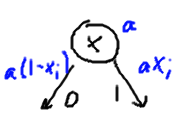
\includegraphics[scale=1.0]{23-7}
\qquad
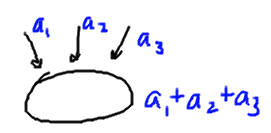
\includegraphics[scale=1.0]{23-8}
\end{figure}
\end{center}

%If we used in terms of arithmetization, 
Using the arithmetization, we can assign non-Boolean values, and there is perhaps some nonsensical result that comes out. Remember that we wrote down the branching program for parity (exclusive or), for instance, $x_1\opl x_2$. Have you ever wondered what $2\opl 3$ is? Probably not. Let's plug in $x_1=2$ and $x_2=3$ into the arithmetized version of this branching program.
%no binary rep.
%\fixme{Fig 9-10.}

Let's see what happens. Plug in 1 at the start node. If we assigned $x_1= 0$ and $x_2=1$, everything work out as before. But now can give values even if we don't have 0's and 1's coming in. We get the following values.

\ig{23-11}{1}

We get $2\opl 3=-7$. (We haven't discovered some fundamental fact about exclusive or. There's no fundamental meaning to this.) %There is an arbitrariness. If we have a different arithmetization you get different values. For this way of representing, we get $-7$. 

Let's summarize. 
Originally we thought of a running a BP as following some path. That way of thinking doesn't lend itself to arithmetization. Instead of thinking about taking a path, think about evaluating a branching program by assigning values to all nodes by the procedure, and looking at 1 node. There is no path, but this way of thinking is  equivalent. We can look at the value on the output node even if the input nodes didn't have 0/1 values coming in.

%in boolean case faithful representation of function. non-boolean case: wacky stuff happening. 1s along path. no path reenter node.

If we had a different branching program representation of the same boolean formula (say, xor), would we get different value? No. As you will see from the coming proof, if we have a different representation that is still read-once, and it agrees on the boolean case, then it agrees on the non-boolean case. This is not true with a general branching program!

As an example, if we flip $x_1,x_2$ in the xor program we get the same value for $2\opl 3$.
%flip x_1,x_2.

%flip 2 and 3. 

%if true in oth branching prog, then prob alg for general bprog, amazing.

Finally, here is the probabilistic algorithm. 

\begin{proof}
Let $M=$``on $\an{B_1,B_2}$,
\begin{enumerate}
\item
Randomly select non-Boolean values for $x_1,\ldots, x_m$ from the finite field $\fq=\{0,1,\ldots, q-1\}$ where $q$ is prime (this is modular arithmetic modulo $q$). Choose $q>3m$.
\item
Compute $B_1,B_2$ (arithmetized) on $x_1,\ldots, x_m$.
\item
\ul{Accept} if we get the same output value.
\ul{Reject} if we do not."
\end{enumerate}
Now we have to prove this works.

We claim the following.
\begin{enumerate}
\item
If $B_1,B_2$ are equivalent then $P(M\text{ accepts})=1$.
(If they agree then they agree on boolean values. We'll prove they agree even on nonboolean values.)
\item
If $B_1,B_2$ are not equivalent then $P(M\text{ rejects})\ge \fc 23$.
\end{enumerate}
We prove statement 1. This is the hard part.
%no more path, no more getting, having trouble letting go

%This comes from
We take the input variables and keep them as variables $x_i$; do the calculation symbolically. %for the proof 
%Leave them as $x_i$'s. 
We'll write down expressions like $x_1$, $1-x_1$, and so forth. At every step we're multiplying things like $x_i$ or $(1-x_i)$, or adding together terms. %and always multiplying by $x_i$ or $(1-x_i)$. 
At the output node 1 we have some polynomial in $x_1,\ldots, x_m$. 

Evaluating $B_1, B_2$ symbolically in the arithmetized version, we get polynomials $P_1,P_2$ on $x_1,\ldots, x_m$. These polynomials have a very nice form: They all look like products of $x_i$'s and $(1-x_i)$'s, added up, for instance %things from diff branches going to same node
\begin{align*}
&\quad x_1(1-x_2)x_3x_4(1-x_5)\cdots x_m\\
&+ (1-x_1)x_2x_3(1-x_4)\cdots \\
&+\cdots.\end{align*}

In each summand, we never get same variable appearing more than once because of the read-once property. %
How do we know we get every variable appearing once? We can always pad out a branching program by adding missing variables, to turn it into a ``read exactly once" branching program. %adding dummy variable.

Both $P_1,P_2$ look like this. Why is it nice? {\it It's the truth table of the original program on Boolean values.} %The top row has value 1 only when every term is 1, and so forth. 
The summands give the rows of the Boolean truth table. If two BP's agree in the Boolean world, they have the same truth table and hence the same polynomial, and agree everywhere.
%The polynomial is equivalent to the Boolean truth table that came from the original branching program. The values on the Boolean case force the rest of the values. They are the same polynomial. 

(There is an exponential number of rows, but this doesn't matter: when we run the algorithm, we don't calculate the polynomial, which takes exponential time. We get a specific value of the polynomial by plugging in values and computing things on the fly.)

Part 2 uses a magical fact about polynomials. 
\begin{lem}
If $P(x)$ is a nonzero polynomial of degree at most $d$, then $P(x)$ has at most $d$ zeros. (This is true in any field, in particular $\fq$.)
\end{lem}
The probabilistic version is the following: if you pick $x\in \fq$ at random, $\Prob(P(x)=0)\le \fc{d}{q}$.
%reasonably low degree, big field, evaluate at random place, chances small it's 0. low degree polys have few roots.
Lemma 2 is the multivariate version.
\begin{lem}[Schwartz-Zippel]\llabel{lem:schwartz-zippel}
If $P(x_1,\ldots, x_m)$ is nonzero, each $x_i$ has degree at most $d$, and you pick $x_i\in \fq$ randomly, then 
\[\Prob[P(x_1,\ldots, x_m)=0]\le \fc{md}{q}.\]
\end{lem}
This is proved from the single-variable case by induction.
%run branching program on 2 random values?

Remember we had 2 polynomials $P_1,P_2$? Let's look at the difference $P:=P_1-P_2$. If the branching programs are not equivalent, then the difference of the polynomials is nonzero. That nonzero polynomial has few roots. $P$ is zero in very few places, so $P_1,P_2$ agree in very few places. When we run the arithmetization of $P_1,P_2$, we're unlikely to get the same value coming out. It's very likely we'll get different values coming out, and very likely we'll reject.

For our $P=P_1-P_2$, what is $d$? Every variable appears once. Hence $d=1$. $m$ is the number of variables, and $q>3m$, so the probability is at most $\rc3$. The chance we got an agreement in $P_1,P_2$ is at most $\rc3$. The chance we get disagreement is at least $\fc 23$.
\end{proof}

\cpbox{Though arithmetization---converting boolean formulas to a polynomial and then running on randomly selected nonboolean formula---we can magnify the chance that a probabilistic algorithm works.}
\vskip0.15in
This is a nice probabilistic algorithm. We'll use this method again in the last two lectures, where we'll prove amazing results about satisfiability using interactive proof systems.